\documentclass{article}

\usepackage[final]{neurips_2023}
\usepackage[utf8]{inputenc}
\usepackage[T1]{fontenc}
\usepackage{hyperref}
\usepackage{url}
\usepackage{booktabs}
\usepackage{amsmath}
\usepackage{graphicx}
\usepackage{caption}
\usepackage{enumitem}
\usepackage{tabularx}
\makeatletter
\renewcommand{\@notice}{}
\makeatother

\title{Orthogonal Finetuning for Chinese Instruction}

\author{
  LU Haodong \\
  1155228939@link.cuhk.edu.hk\\
  Department of Computer Science and Engineering\\
  The Chinese University of Hong Kong
}

\begin{document}
\maketitle
\noindent\textbf{Project repository:} \url{https://github.com/SleepyLGod/mini-oft-llm.git}

\section{Introduction}
This report studies Orthogonal Finetuning (OFT) for Chinese instruction-following supervised finetuning on \texttt{Qwen2.5-7B-Instruct}. The assignment requires training-loss curves and final quantitative and/or before-vs-after qualitative outcomes. The report is designed to satisfy those requirements with evidence-driven claims only.

\textbf{Background and motivation.} OFT applies multiplicative orthogonal updates, offering a parameter-efficient alternative to additive low-rank adaptation such as LoRA \citep{qiu2023oft,hu2021lora}. The motivation is to improve instruction behavior under fixed compute and limited training window, while avoiding full-parameter finetuning cost. In practical terms, this work asks whether a constrained OFT update can produce robust in-domain gains without expanding adaptation complexity.

\textbf{Experiment objectives.} Effectiveness-wise, we want to measure in-domain likelihood improvement of OFT over the frozen base model. Sensitivity-wise, we want to compare \texttt{oft\_block\_size=32} against \texttt{16} under matched setup.

The report evaluates both objectives using quantitative and qualitative evidence jointly: token-level likelihood for global trend, and fixed prompts for behavioral strengths/failures. This combination is important because single-number improvement does not guarantee uniform instruction-following quality.

\section{Experimental Design and Implementation}
\textbf{Data.} A Chinese instruction corpus is used with fixed split and seed. Final split sizes are 1,484,455 (train), 82,465 (validation), and 82,479 (test), totaling 1,649,399 samples \citep{firefly_dataset}.

\textbf{Model and compute.} The base model is Qwen2.5-7B-Instruct \citep{qwen25_report}. Training is distributed over 2$\times$H100 NVL in bf16.

\textbf{Training setup.} Main run and ablation run both use 1200 steps with matched optimizer/scheduler/batch settings. OFT is applied to all linear modules with Cayley-Neumann enabled. The only ablated variable is \texttt{oft\_block\_size} (32 vs.\ 16).

Instruction tuning is implemented as causal language-model SFT with unified sequence formatting, so all compared runs optimize the same objective on the same tokenization regime. This removes task-definition confounders from the ablation comparison.

\textbf{Implementation pipeline details.} The workflow is fixed to reduce execution risk: deterministic preprocessing, a 100-step distributed smoke run, two matched full runs (main and ablation), and a shared evaluator on the same 2000-sample test slice. Quantitative metrics and before/after generations are then consolidated for consistency checks between likelihood gains and behavior changes.

\textbf{Evaluation protocol.} Three evidence channels are used:
\begin{itemize}[leftmargin=*]
  \item token-level NLL and PPL on a fixed 2000-sample test slice,
  \item final validation \texttt{eval\_loss},
  \item fixed-prompt before/after generations.
\end{itemize}
Cross-run \texttt{train\_loss} is not treated as primary comparison evidence because resumed-run behavior affects direct comparability.

This protocol separates optimization signal (NLL/PPL and \texttt{eval\_loss}) from user-facing behavior (prompt-level quality).

\section{Results and Analysis}
\begin{table}[t]
  \centering
  \caption{Primary quantitative results on 2000 held-out samples (lower is better). The table supports in-domain likelihood comparison, not out-of-domain generalization claims.}
  \label{tab:main_results}
  \resizebox{\linewidth}{!}{
  \begin{tabular}{lccccc}
      \toprule
      Model & Mean NLL & PPL & $\Delta$NLL vs Base & $\Delta$PPL vs Base & eval\_loss \\
      \midrule
      Base (no finetuning) & 3.2619 & 26.0990 & -- & -- & -- \\
      OFT main (\texttt{block\_size=32}) & \textbf{1.9770} & \textbf{7.2207} & \textbf{-39.39\%} & \textbf{-72.33\%} & \textbf{1.7879} \\
      OFT ablation (\texttt{block\_size=16}) & 1.9988 & 7.3803 & -38.72\% & -71.72\% & 1.8102 \\
      \bottomrule
  \end{tabular}
  }
\end{table}

OFT (main) improves over base by 39.39\% in NLL and 72.33\% in PPL. Against ablation, \texttt{block\_size=32} improves by 1.09\% in NLL and 2.16\% in PPL (relative). The strongest quantitative highlight is the large base-to-OFT gap under fixed compute budget.

\begin{figure*}[t]
  \centering
  
\includegraphics[width=0.96\textwidth]{figures/loss_comparison.png}
  \caption{Training and validation loss comparison. Both runs converge stably, and \texttt{block\_size=32} finishes with lower validation loss.}
  \label{fig:main_figs}
\end{figure*}

\begin{figure}[t]
  \centering
  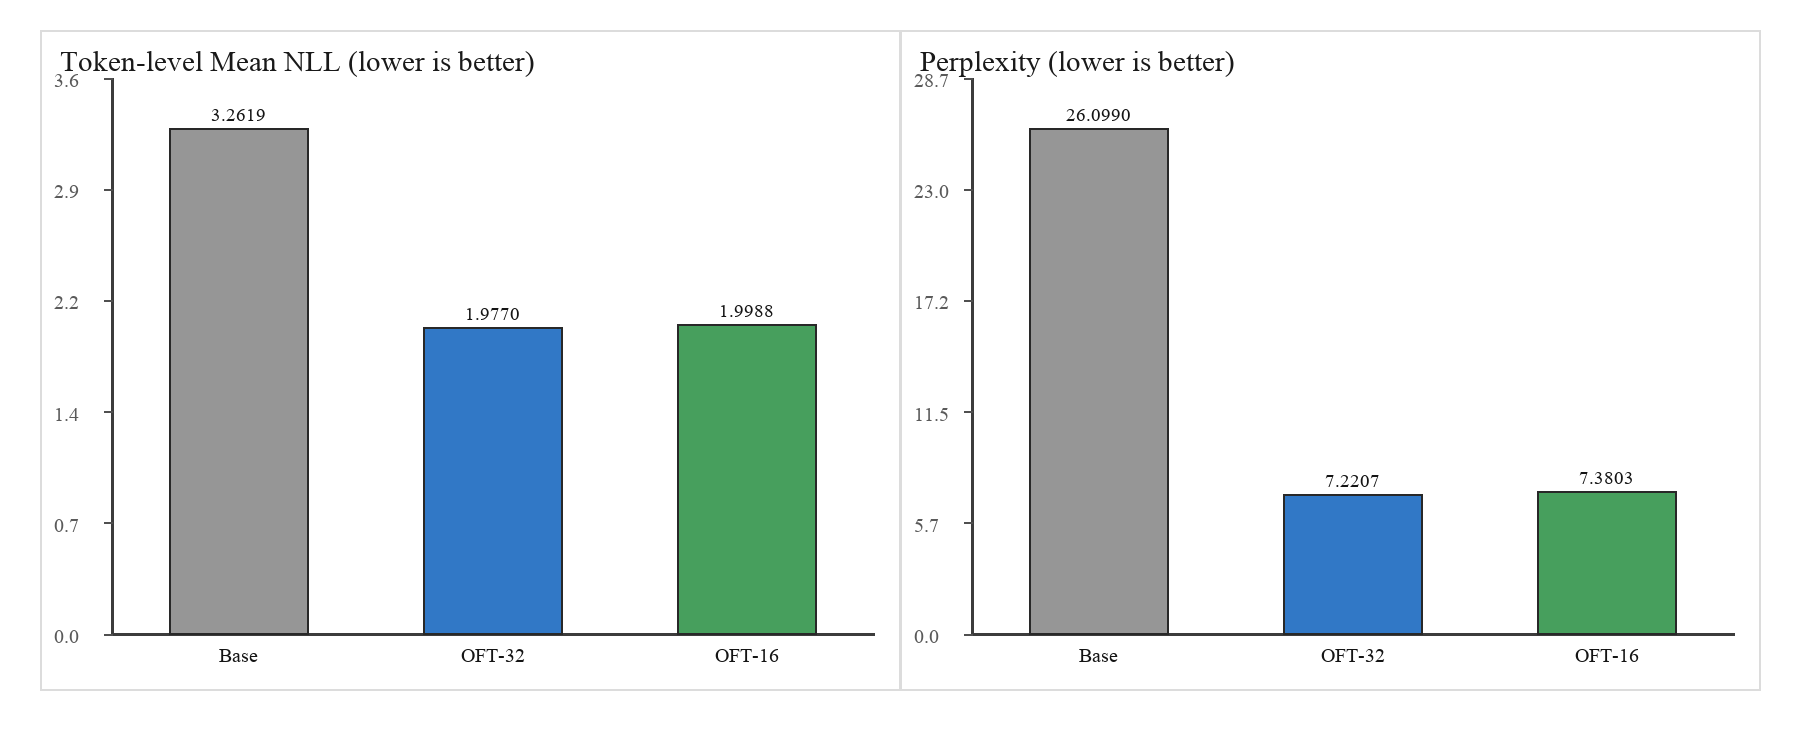
\includegraphics[width=0.96\linewidth,height=0.20\textheight,keepaspectratio]{figures/metric_bars.png}
  \caption{Token-level NLL/PPL bars for base, main, and ablation, showing a large base-to-OFT gap and a smaller but consistent main-vs-ablation gap.}
  \label{fig:metric_bars}
\end{figure}

\begin{table*}[t]
  \centering
  \scriptsize
  \caption{Representative before-vs-after qualitative evidence with improvements, regressions, and tradeoff behavior.}
  \label{tab:qual_cases}
  {
  \setlength{\tabcolsep}{4pt}
  \resizebox{\textwidth}{!}{
  \begin{tabular}{lllll}
      \toprule
      Prompt ID & Task & Outcome & Base snippet & OFT snippet \\
      \midrule
      P007 & Classification & Improved & Explanatory sentence around sentiment. & Label-only output matching requested format. \\
      P010 & Extraction & Improved & Verbose extraction with surrounding explanation. & Compact field lines: location / time / person. \\
      P033 & Safety & Improved & Long risk explanation and general advice. & Direct refusal plus concise safe redirection. \\
      P025 & Coding & Tradeoff & Correct code with extra explanation/tests. & Correct concise function, less pedagogy. \\
      P016 & Reasoning & Regressed & Multi-step operational incident response. & Short checklist bullets with less depth. \\
      P042 & Instruction-following & Regressed & Three-line fruit list (format correct). & One-line comma-separated output (format wrong). \\
      P045 & Domain explanation & Regressed & Multi-point rationale for canary release value. & Single-sentence compressed summary. \\
      \bottomrule
  \end{tabular}
  }
  }
\end{table*}

\textbf{Integrated discussion.} Gains are task-dependent: concise constrained tasks improve clearly, while reasoning depth and strict format compliance may regress.

\textbf{Structured analysis (P1/P2/P3).}
\begin{itemize}[leftmargin=*]
  \item \textbf{P1: Primary effectiveness signal.} Under fixed compute and split, OFT shows a large in-domain gain over base (NLL 3.2619 $\rightarrow$ 1.9770; PPL 26.0990 $\rightarrow$ 7.2207), consistent across table metrics and curve trends.
  \item \textbf{P2: Robustness under constrained ablation.} With matched settings, \texttt{block\_size=32} stays better than \texttt{16} (NLL -1.09\%, PPL -2.16\%, and lower \texttt{eval\_loss}); the margin is modest but directionally stable.
  \item \textbf{P3: Behavioral tradeoff and deployment implication.} Concise structured tasks improve (P007/P010/P033), while format-critical or depth-demanding prompts can regress (P016/P042/P045), suggesting extra guardrails for strict-format and reasoning-depth use cases.
\end{itemize}

\section{Limitations and Conclusion}
\textbf{Limitations.}
\begin{itemize}[leftmargin=*]
  \item Evaluation is in-domain; broad transfer claims are unsupported.
  \item Potential near-duplicate overlap can inflate measured gains.
  \item NLL/PPL do not fully capture preference quality, factuality, or strict format reliability.
  \item Qualitative evidence is representative but not exhaustive.
\end{itemize}

These results should be interpreted as \emph{task- and distribution-scoped} rather than universal model improvement.

\textbf{Conclusion.}
\begin{itemize}[leftmargin=*]
  \item OFT achieves strong in-domain likelihood improvement over the frozen base model.
  \item \texttt{oft\_block\_size=32} outperforms \texttt{16} across tracked primary metrics.
  \item The main practical tradeoff is improved conciseness vs.\ occasional depth/format regressions.
\end{itemize}

\paragraph{Instruction alignment statement.}
This report includes all required evidence: training-loss curves (Figure~\ref{fig:main_figs}), final quantitative performance (Table~\ref{tab:main_results}), and before-vs-after qualitative outcomes (Table~\ref{tab:qual_cases}).

{\footnotesize
\bibliographystyle{plainnat}
\bibliography{references}
}

\end{document}
